\documentclass[12pt, letterpaper]{report}
\usepackage{datetime}
\newdateformat{monthyeardate}{\monthname[\THEMONTH] \THEYEAR}

\title{\textbf{ECS 132 Term Project}}
\author{\parbox{\linewidth}{\centering%
  Steven Alvarado, Russell Chien, and Ruth Hailu\endgraf\bigskip
  University of California, Davis}}
\date{\monthyeardate\today}

\usepackage{graphicx} 
\usepackage{titlesec}
\usepackage{amsmath}
\usepackage{listings}
\usepackage[usenames,dvipsnames]{color} 

\lstset{ 
  language=R,                     % the language of the code
  basicstyle=\normalsize\ttfamily, % the size of the fonts that are used for the code
  numbers=left,                   % where to put the line-numbers
  numberstyle=\normalsize\color{Blue},  % the style that is used for the line-numbers
  stepnumber=1,                   % the step between two line-numbers. If it is 1, each line
                                  % will be numbered
  numbersep=5pt,                  % how far the line-numbers are from the code
  backgroundcolor=\color{white},  % choose the background color. You must add \usepackage{color}
  showspaces=false,               % show spaces adding particular underscores
  showstringspaces=false,         % underline spaces within strings
  showtabs=false,                 % show tabs within strings adding particular underscores
  frame=single,                   % adds a frame around the code
  rulecolor=\color{black},        % if not set, the frame-color may be changed on line-breaks within not-black text (e.g. commens (green here))
  tabsize=2,                      % sets default tabsize to 2 spaces
  captionpos=b,                   % sets the caption-position to bottom
  breaklines=true,                % sets automatic line breaking
  breakatwhitespace=false,        % sets if automatic breaks should only happen at whitespace
  keywordstyle=\color{RoyalBlue},      % keyword style
  commentstyle=\color{YellowGreen},   % comment style
  stringstyle=\color{ForestGreen}      % string literal style
} 

\graphicspath{{plots/}}

\titleformat{\chapter}[display]
  {\normalfont\huge\bfseries\filcenter}{\chaptertitlename\ \thechapter}{20pt}{\Huge}
\titlespacing*{\chapter}
  {0pt}{30pt}{20pt}

\begin{document}
\maketitle
\chapter{The Normal Family}
\section{Communities and Crime: pctWWage}

Our group observed that the variable \textbf{pctWWage} of the Communities and Crime dataset seemed well-approximated by the normal family of continuous distributions.
According to the UCI Machine Learning Repository, \textbf{pctWWage} is described as the percentage of households within the United States with wage or salary income in 1989.

\section{Histogram and Density}


\begin{center}
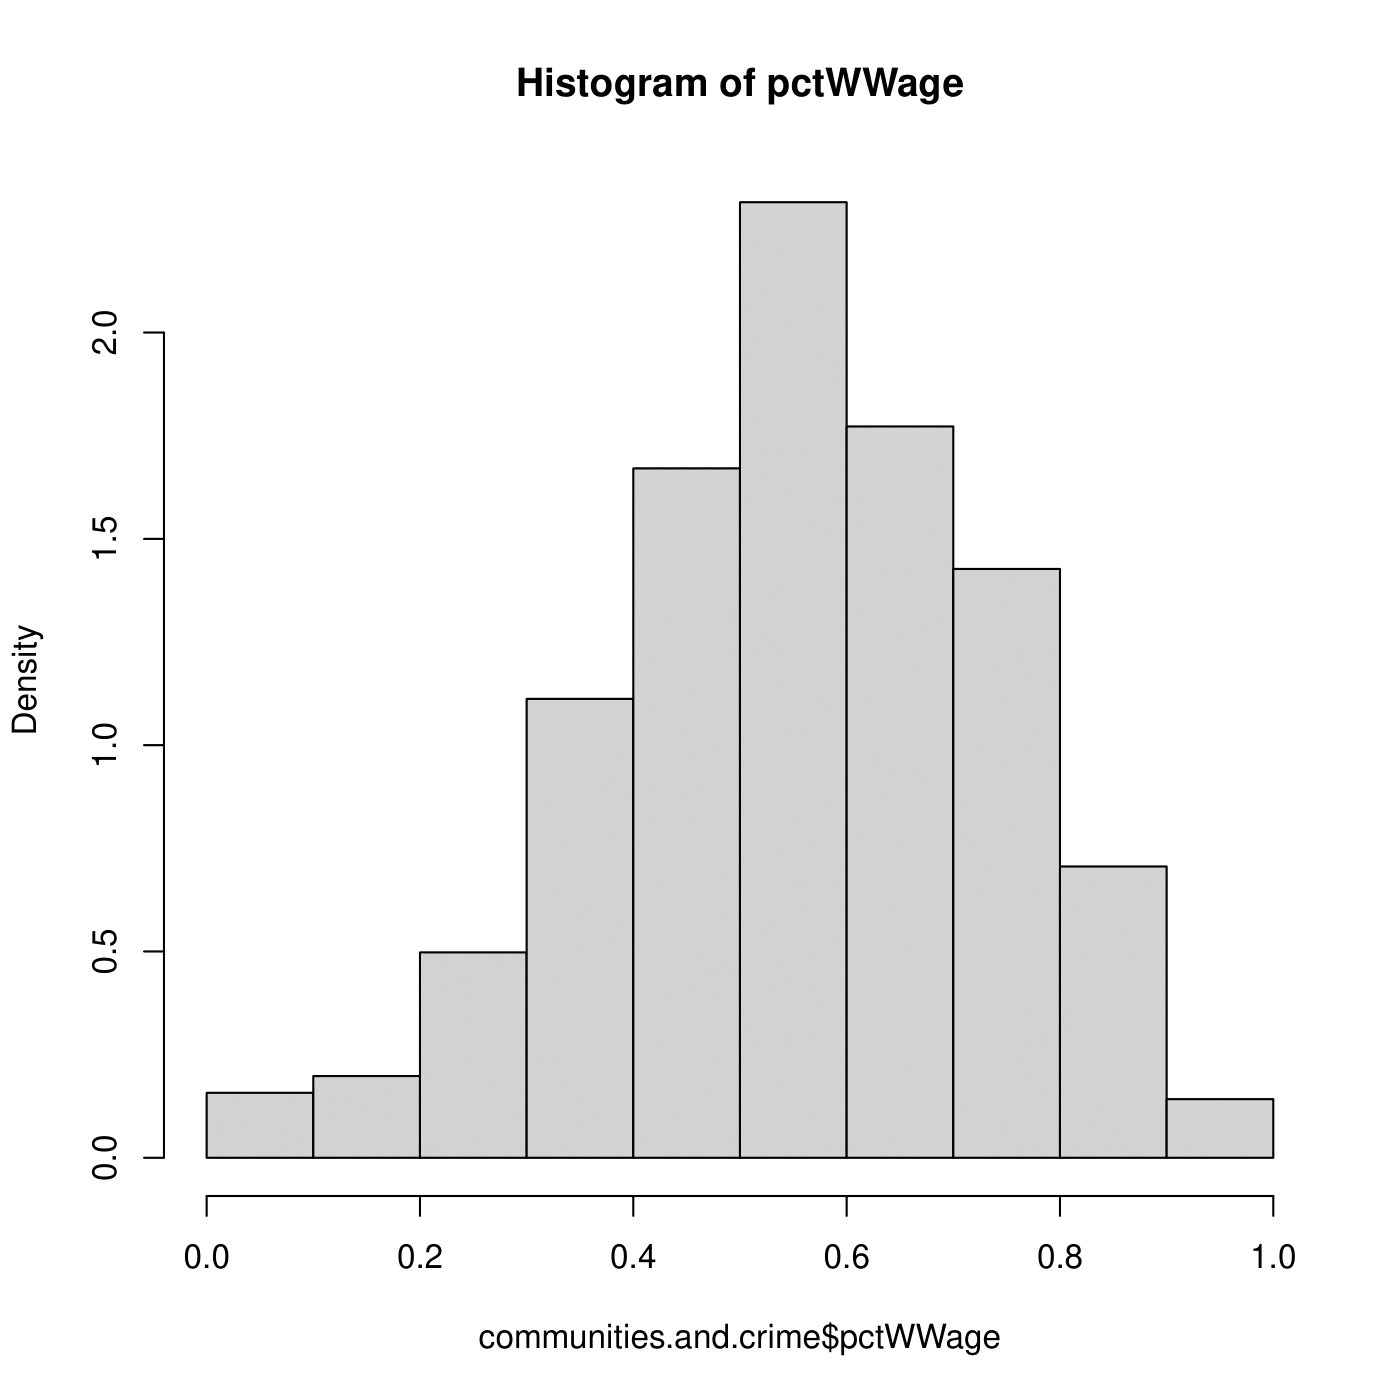
\includegraphics[width=0.45\textwidth]{normal/pctWWage_hist}
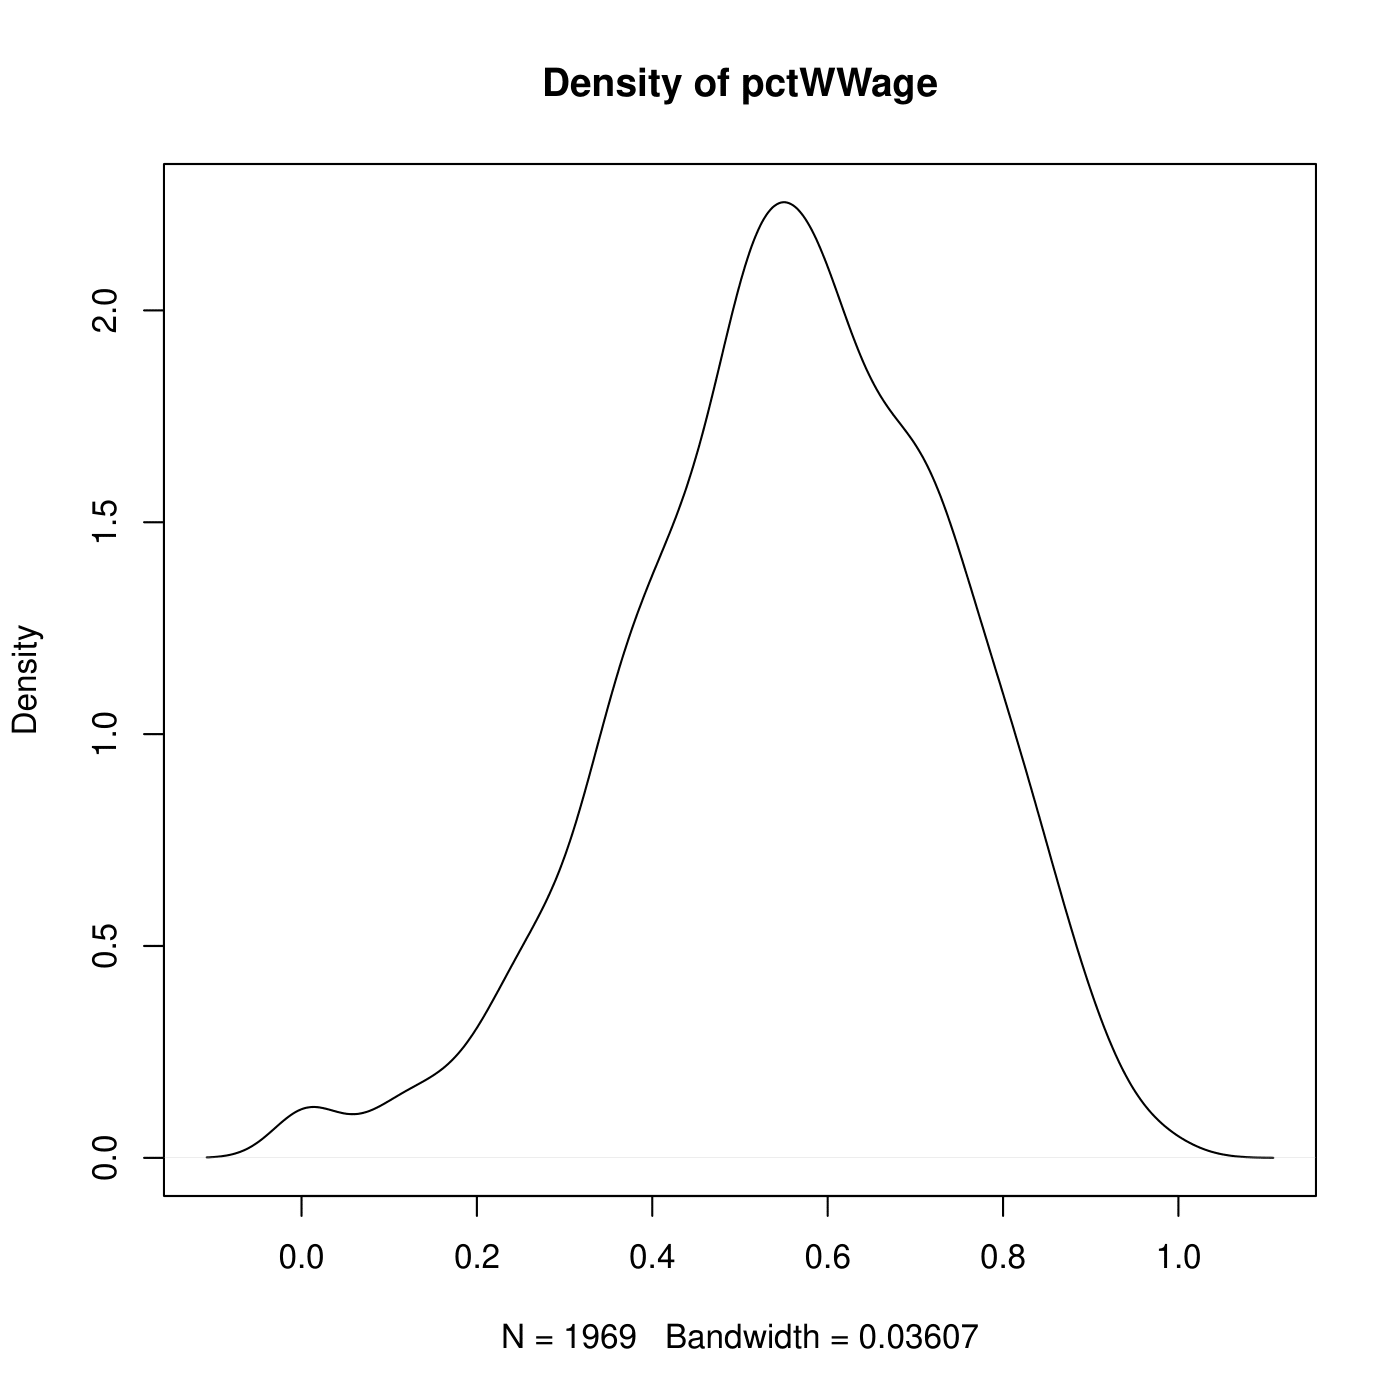
\includegraphics[width=0.45\textwidth]{normal/pctWWage_density}
\end{center}


\section{MLE and MM}


\begin{center}
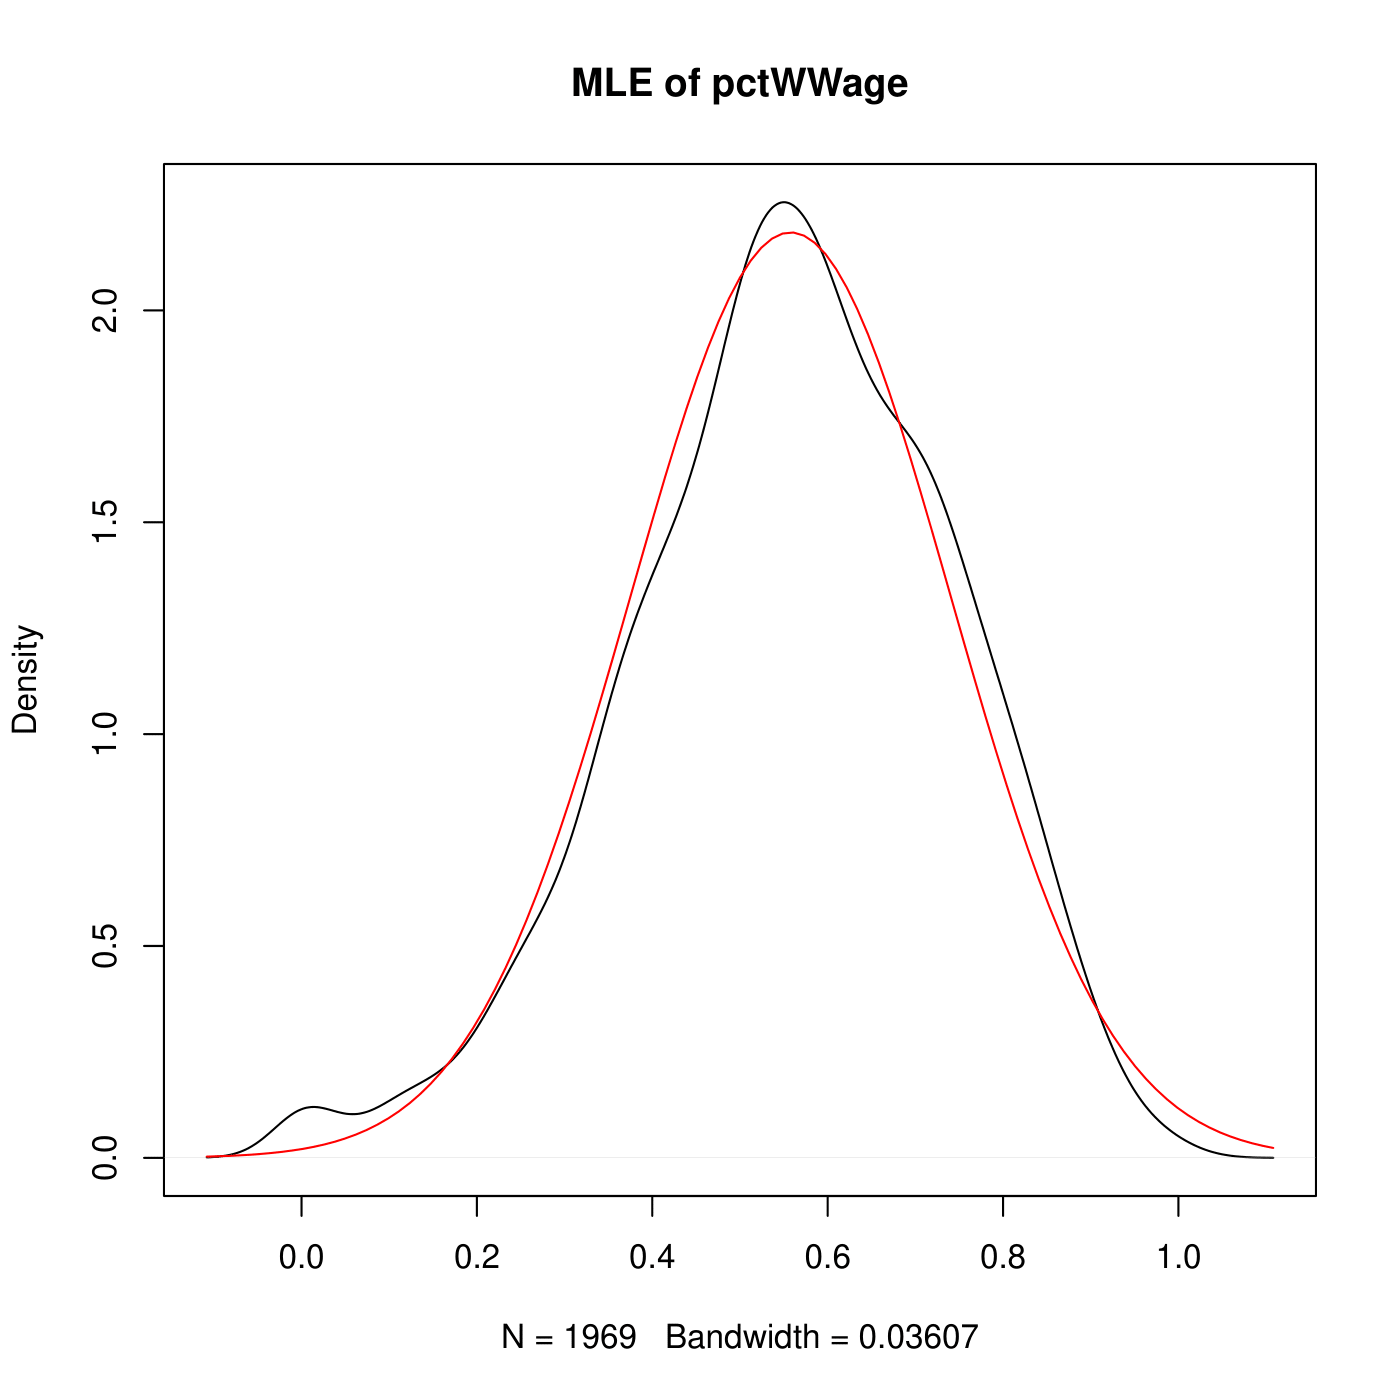
\includegraphics[width=0.45\textwidth]{normal/pctWWage_mle}
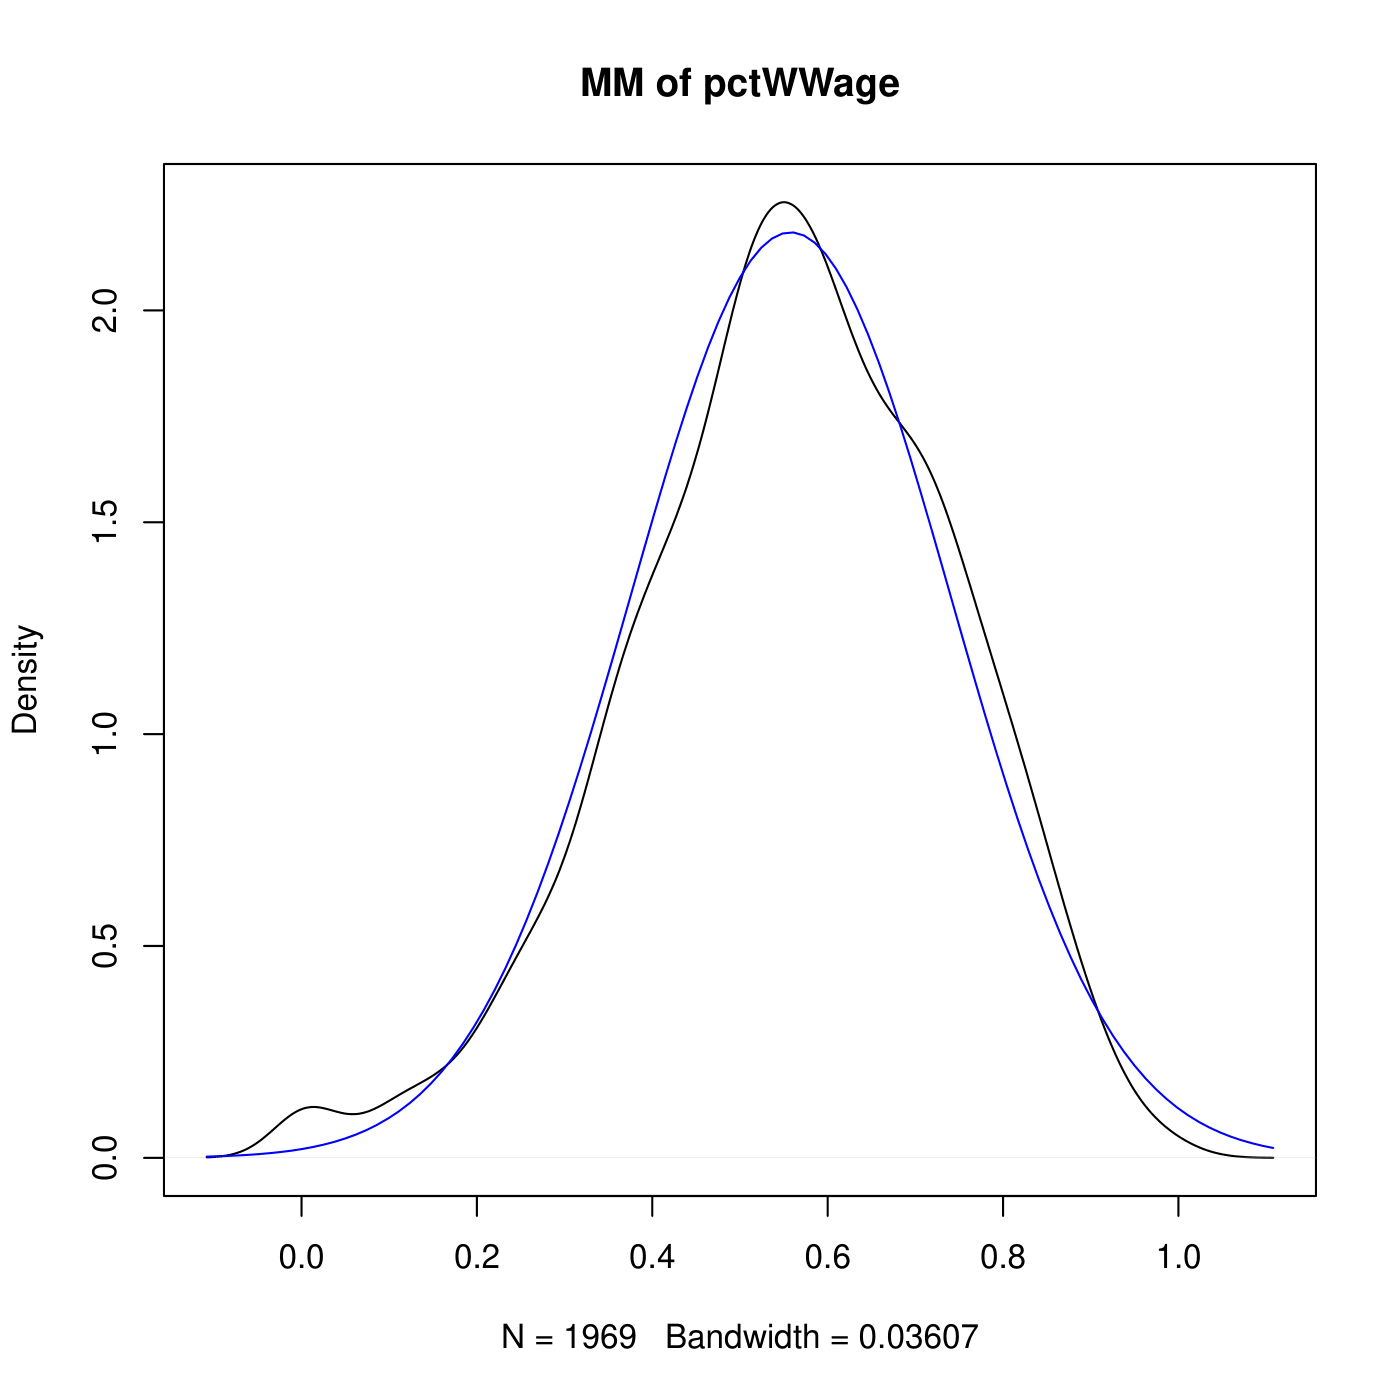
\includegraphics[width=0.45\textwidth]{normal/pctWWage_mm}
\end{center}

\section{Conclusion}


\maketitle
\chapter{The Exponential Family}
\section{Communities and Crime: PctLargHouseFam}

For the exponential family of continuous distributions, we observed that the variable \textbf{PctLargHouseFam} was a suitable approximation. 
According to the UCI Machine Learning Repository, \textbf{PctLargHouseFam} is described as the percentage of family households with six or more family members. 

\section{Histogram and Density}


\begin{center}
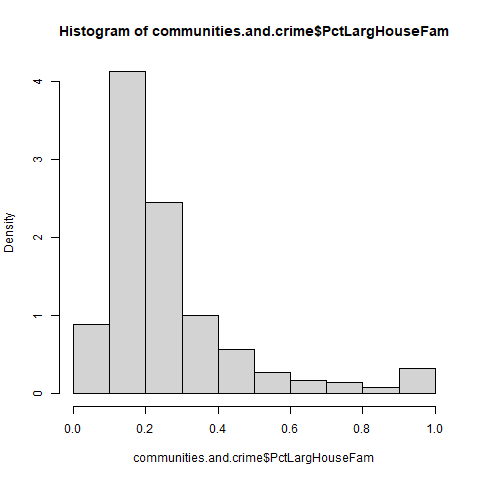
\includegraphics[width=0.45\textwidth]{exponential/PctLargHouseFam_hist}
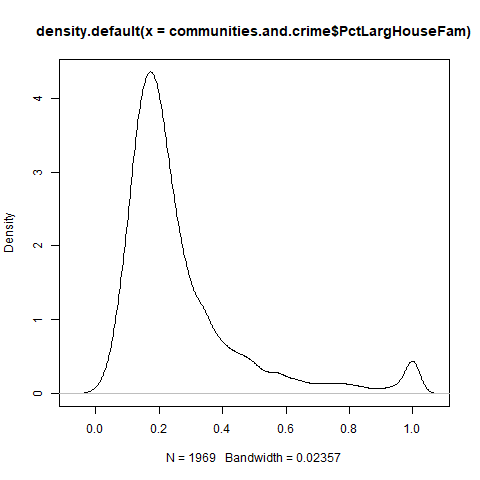
\includegraphics[width=0.45\textwidth]{exponential/PctLargHouseFam_density}
\end{center}

\section{MLE and MM}


\begin{center}
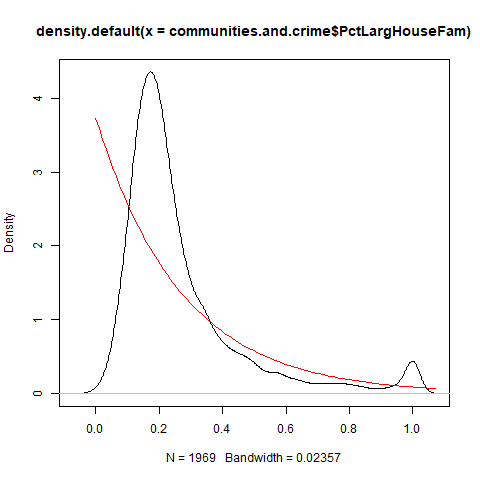
\includegraphics[width=0.45\textwidth]{exponential/PctLargHouseFam_mle}
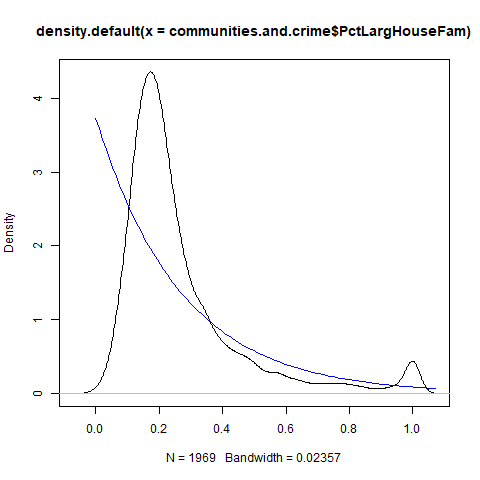
\includegraphics[width=0.45\textwidth]{exponential/PctLargHouseFam_mm}
\end{center}

\section{Conclusion}


\maketitle
\chapter{The Gamma Family}
\section{Communities and Crime: PctNotHsGrad}

We observed that the variable \textbf{PctNotHsGrad} of the Communities and Crime dataset seemed well-approximated by the gamma family of continuous distributions.
According to the UCI Machine Learning Repository, \textbf{PctNotHsGrad} is described as the percentage of people 25 and over that are not high school graduates.


\section{Histogram and Density}


\begin{center}
\includegraphics[width=0.45\textwidth]{gamma/PctNotHsGrad_hist}
\includegraphics[width=0.45\textwidth]{gamma/PctNotHsGrad_density}
\end{center}

\section{MLE and MM}


\begin{center}
\includegraphics[width=0.45\textwidth]{gamma/PctNotHsGrad_mle}
\includegraphics[width=0.45\textwidth]{gamma/PctNotHsGrad_mm}
\end{center}

\section{Conclusion}


\maketitle
\chapter{The Beta Family}
\section{Communities and Crime: PctNotSpeakEnglWell}

For the beta family of continuous distributions, we observed that the variable \textbf{PctNotSpeakEnglWell} was a suitable approximation. 
According to the UCI Machine Learning Repository, \textbf{PctNotSpeakEnglWell} is described as the percentage of people who do not speak English well. 


\section{Histogram and Density}


\begin{center}
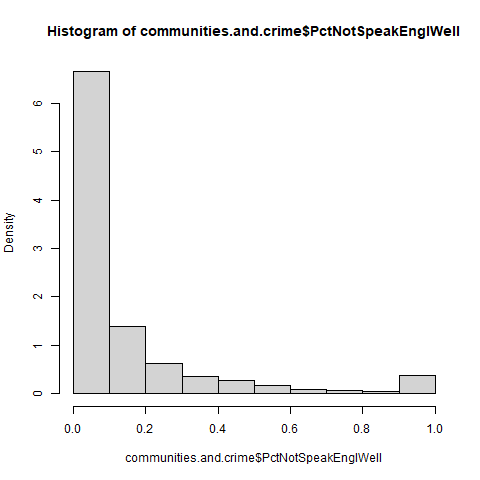
\includegraphics[width=0.45\textwidth]{beta/PctNotSpeakEnglWell_hist}
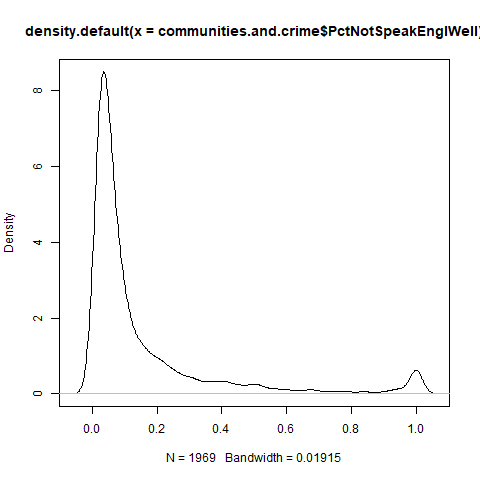
\includegraphics[width=0.45\textwidth]{beta/PctNotSpeakEnglWell_density}
\end{center}


\section{MLE and MM}
To find the MLE of the beta family, we first had to scale our data so it was within the support of $(0, 1)$: 
\begin{lstlisting}
  x[which(x == 0)] <- 0.0001  
  x[which(x == 1)] <- 0.9999
\end{lstlisting} 
We then found the log likelihood function:
\begin{multline}
L(\alpha, \beta) = n \log{(\Gamma(\alpha+\beta))} - n \log{(\Gamma(\alpha))} - n \log{(\Gamma(\beta))} + \\
(\alpha - 1) \sum(\log(x)) + (\beta-1) \sum(\log{(1-x)})
\end{multline}
To find the MLE, we use R's built in mle() function with the negative value of our 4.1 log likelihood function. 
\begin{lstlisting}
z <- mle(minuslogl = ll, start = c(list(alpha = 1), list(beta = 1)))
\end{lstlisting} 

\begin{center}
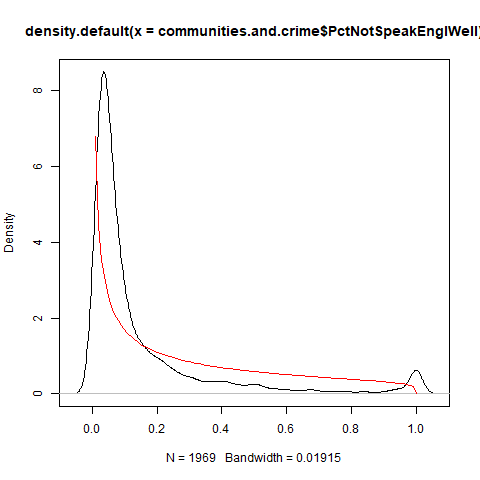
\includegraphics[width=0.45\textwidth]{beta/PctNotSpeakEnglWell_mle}
\end{center}

To find the MM of the beta family, we used the following function to estimate the $\alpha$ and $\beta$ values:
\begin{lstlisting}
  mm <- function(x) {
    mu <- mean(x)
    var <- var(x)
    alpha <- mu * (mu * (1 - mu) / var - 1)
    beta <- (1 - mu) * (mu * (1 - mu) / var - 1)
    return(c(alpha, beta))
}
\end{lstlisting} 

\begin{center}
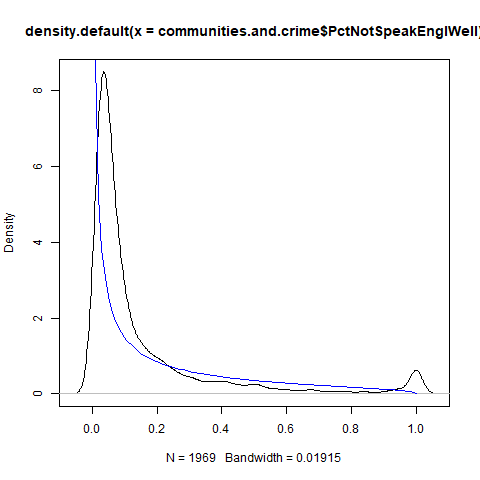
\includegraphics[width=0.45\textwidth]{beta/PctNotSpeakEnglWell_mm}
\end{center}

\section{Conclusion}

\end{document}